\documentclass[11pt,preprint, authoryear]{elsarticle}

\usepackage{lmodern}
%%%% My spacing
\usepackage{setspace}
\setstretch{1.2}
\DeclareMathSizes{12}{14}{10}{10}

% Wrap around which gives all figures included the [H] command, or places it "here". This can be tedious to code in Rmarkdown.
\usepackage{float}
\let\origfigure\figure
\let\endorigfigure\endfigure
\renewenvironment{figure}[1][2] {
    \expandafter\origfigure\expandafter[H]
} {
    \endorigfigure
}

\let\origtable\table
\let\endorigtable\endtable
\renewenvironment{table}[1][2] {
    \expandafter\origtable\expandafter[H]
} {
    \endorigtable
}


\usepackage{ifxetex,ifluatex}
\usepackage{fixltx2e} % provides \textsubscript
\ifnum 0\ifxetex 1\fi\ifluatex 1\fi=0 % if pdftex
  \usepackage[T1]{fontenc}
  \usepackage[utf8]{inputenc}
\else % if luatex or xelatex
  \ifxetex
    \usepackage{mathspec}
    \usepackage{xltxtra,xunicode}
  \else
    \usepackage{fontspec}
  \fi
  \defaultfontfeatures{Mapping=tex-text,Scale=MatchLowercase}
  \newcommand{\euro}{€}
\fi

\usepackage{amssymb, amsmath, amsthm, amsfonts}

\def\bibsection{\section*{References}} %%% Make "References" appear before bibliography


\usepackage[round]{natbib}

\usepackage{longtable}
\usepackage[margin=2.3cm,bottom=2cm,top=2.5cm, includefoot]{geometry}
\usepackage{fancyhdr}
\usepackage[bottom, hang, flushmargin]{footmisc}
\usepackage{graphicx}
\numberwithin{equation}{section}
\numberwithin{figure}{section}
\numberwithin{table}{section}
\setlength{\parindent}{0cm}
\setlength{\parskip}{1.3ex plus 0.5ex minus 0.3ex}
\usepackage{textcomp}
\renewcommand{\headrulewidth}{0.2pt}
\renewcommand{\footrulewidth}{0.3pt}

\usepackage{array}
\newcolumntype{x}[1]{>{\centering\arraybackslash\hspace{0pt}}p{#1}}

%%%%  Remove the "preprint submitted to" part. Don't worry about this either, it just looks better without it:
\makeatletter
\def\ps@pprintTitle{%
  \let\@oddhead\@empty
  \let\@evenhead\@empty
  \let\@oddfoot\@empty
  \let\@evenfoot\@oddfoot
}
\makeatother

 \def\tightlist{} % This allows for subbullets!

\usepackage{hyperref}
\hypersetup{breaklinks=true,
            bookmarks=true,
            colorlinks=true,
            citecolor=blue,
            urlcolor=blue,
            linkcolor=blue,
            pdfborder={0 0 0}}


% The following packages allow huxtable to work:
\usepackage{siunitx}
\usepackage{multirow}
\usepackage{hhline}
\usepackage{calc}
\usepackage{tabularx}
\usepackage{booktabs}
\usepackage{caption}


\newenvironment{columns}[1][]{}{}

\newenvironment{column}[1]{\begin{minipage}{#1}\ignorespaces}{%
\end{minipage}
\ifhmode\unskip\fi
\aftergroup\useignorespacesandallpars}

\def\useignorespacesandallpars#1\ignorespaces\fi{%
#1\fi\ignorespacesandallpars}

\makeatletter
\def\ignorespacesandallpars{%
  \@ifnextchar\par
    {\expandafter\ignorespacesandallpars\@gobble}%
    {}%
}
\makeatother

\newlength{\cslhangindent}
\setlength{\cslhangindent}{1.5em}
\newenvironment{CSLReferences}%
  {\setlength{\parindent}{0pt}%
  \everypar{\setlength{\hangindent}{\cslhangindent}}\ignorespaces}%
  {\par}


\urlstyle{same}  % don't use monospace font for urls
\setlength{\parindent}{0pt}
\setlength{\parskip}{6pt plus 2pt minus 1pt}
\setlength{\emergencystretch}{3em}  % prevent overfull lines
\setcounter{secnumdepth}{5}

%%% Use protect on footnotes to avoid problems with footnotes in titles
\let\rmarkdownfootnote\footnote%
\def\footnote{\protect\rmarkdownfootnote}
\IfFileExists{upquote.sty}{\usepackage{upquote}}{}

%%% Include extra packages specified by user

%%% Hard setting column skips for reports - this ensures greater consistency and control over the length settings in the document.
%% page layout
%% paragraphs
\setlength{\baselineskip}{12pt plus 0pt minus 0pt}
\setlength{\parskip}{12pt plus 0pt minus 0pt}
\setlength{\parindent}{0pt plus 0pt minus 0pt}
%% floats
\setlength{\floatsep}{12pt plus 0 pt minus 0pt}
\setlength{\textfloatsep}{20pt plus 0pt minus 0pt}
\setlength{\intextsep}{14pt plus 0pt minus 0pt}
\setlength{\dbltextfloatsep}{20pt plus 0pt minus 0pt}
\setlength{\dblfloatsep}{14pt plus 0pt minus 0pt}
%% maths
\setlength{\abovedisplayskip}{12pt plus 0pt minus 0pt}
\setlength{\belowdisplayskip}{12pt plus 0pt minus 0pt}
%% lists
\setlength{\topsep}{10pt plus 0pt minus 0pt}
\setlength{\partopsep}{3pt plus 0pt minus 0pt}
\setlength{\itemsep}{5pt plus 0pt minus 0pt}
\setlength{\labelsep}{8mm plus 0mm minus 0mm}
\setlength{\parsep}{\the\parskip}
\setlength{\listparindent}{\the\parindent}
%% verbatim
\setlength{\fboxsep}{5pt plus 0pt minus 0pt}



\begin{document}



\begin{frontmatter}  %

\title{Question One}

% Set to FALSE if wanting to remove title (for submission)




\author[Add1]{Jessica Van der Berg}
\ead{20190565@sun.ac.za}





\address[Add1]{Financial Econometrics 2021}


\begin{abstract}
\small{
This document contains the detailed answers for question one of the
Financial Econometric exam 2021.
}
\end{abstract}

\vspace{1cm}


\begin{keyword}
\footnotesize{
Question1 \sep Finance\sep Financial Econometrics \\
\vspace{0.3cm}
}
\footnotesize{
\textit{JEL classification} L250 \sep L100
}
\end{keyword}



\vspace{0.5cm}

\end{frontmatter}



%________________________
% Header and Footers
%%%%%%%%%%%%%%%%%%%%%%%%%%%%%%%%%
\pagestyle{fancy}
\chead{}
\rhead{}
\lfoot{}
\rfoot{\footnotesize Page \thepage}
\lhead{}
%\rfoot{\footnotesize Page \thepage } % "e.g. Page 2"
\cfoot{}

%\setlength\headheight{30pt}
%%%%%%%%%%%%%%%%%%%%%%%%%%%%%%%%%
%________________________

\headsep 35pt % So that header does not go over title




\hypertarget{question-1-yeild-spread}{%
\section{\texorpdfstring{Question 1 Yeild Spread
\label{Introduction}}{Question 1 Yeild Spread }}\label{question-1-yeild-spread}}

Question 1 requires an analysis of South Africa's Yield Spreads and
local mid to longer dated yields bonds. There have been claims that the
bond yields are the highest they have been in decades. The plot below
confirms this. As seen in the graph, the lowest spread between the local
bond market was during the 2007/2008 financial crises, afterwhich it
dramatically increases in 2010. The dramatic increase was short lived,
with the yield spread increasing slowly between 2011 and 2019. In 2020,
the yield spread between the 10 Year and 2 year, as well as the yield
spread between the 10 year and 3 month local bonds increased
dramatically. The yield spread between the 2 year and 3 month local
bonds also experienced an increase, however, this increase reached
levels similar to those experienced in 2000/2001.

In increase in the yield spread can be explained by the uncertainty in
the markets during the still on-going COVID-19 pandemic. Investors
rushed to raise liquidity amid the uncertainty and panic, particularly
those regarded as having a hint of risk. South African government bonds
did not escape the effect of the pandemic, with significant sales of the
asset class by foreigners, causing yields to spike and prices to move
lower.

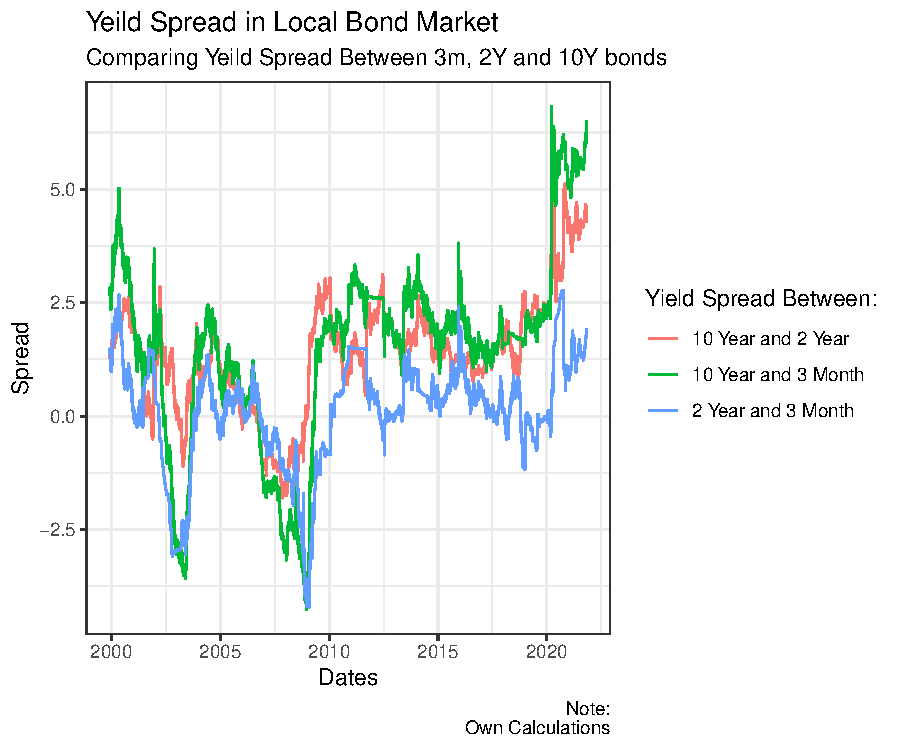
\includegraphics{Question1_files/figure-latex/unnamed-chunk-1-1.pdf}

This effect felt are not isolated to the South African bond market, with
all emerging market local currency debt selling off in unison, as will
be shown in the graphs below. This graph follows a similar pattern ad
the local bonds yeild spread.

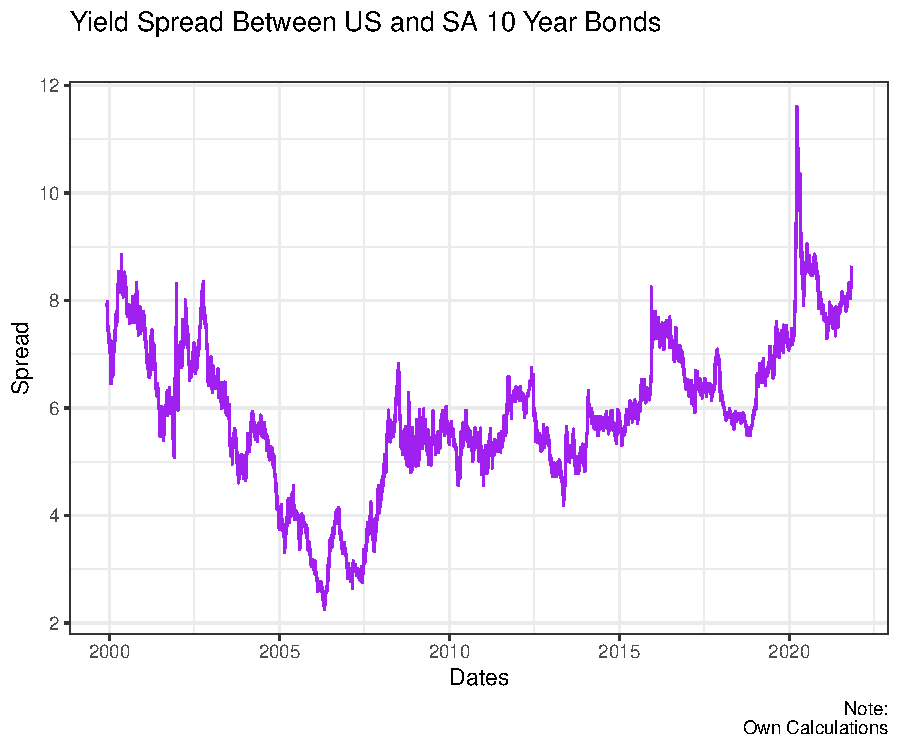
\includegraphics{Question1_files/figure-latex/unnamed-chunk-2-1.pdf}

\hypertarget{usdzar-level}{%
\subsection{USD/ZAR level}\label{usdzar-level}}

The spreads of the 10-year bond yields can be used to gauge currencies.
The general rule is that when the yield spread widens in favor of a
certain currency, that currency will appreciate against other
currencies.

Yield spreads are often seen as driven by monetary policy. Differences
in the exchange rate will drastically affect the expected yield. The
graph below shows that this is true for longer term bonds, however,
there is more volatility is shorter term bonds implying that the
exchange rate is not that good of a predictor and that monetary policy
changes will drastically affect the yield.

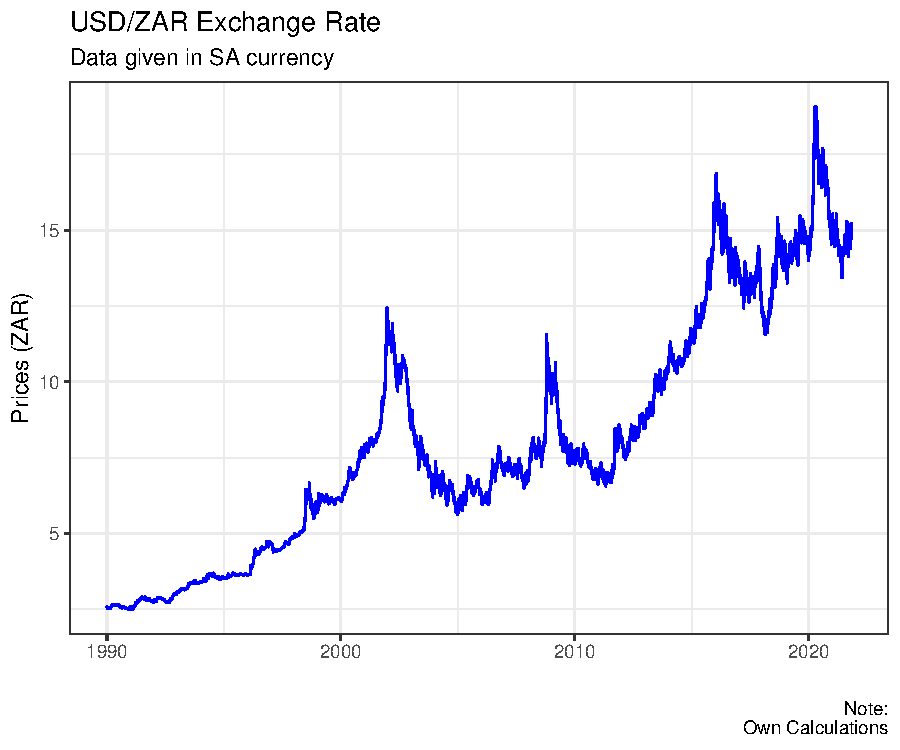
\includegraphics{Question1_files/figure-latex/unnamed-chunk-3-1.pdf}

\hypertarget{different-yeild-spreads}{%
\subsection{Different Yeild Spreads}\label{different-yeild-spreads}}

Comparing the 10 year and 2 year bond is important, so that investor can
determine whether a bond is fairly priced, cheap or expensive. It is a
sign of the risk premium for investing in one investment over another.

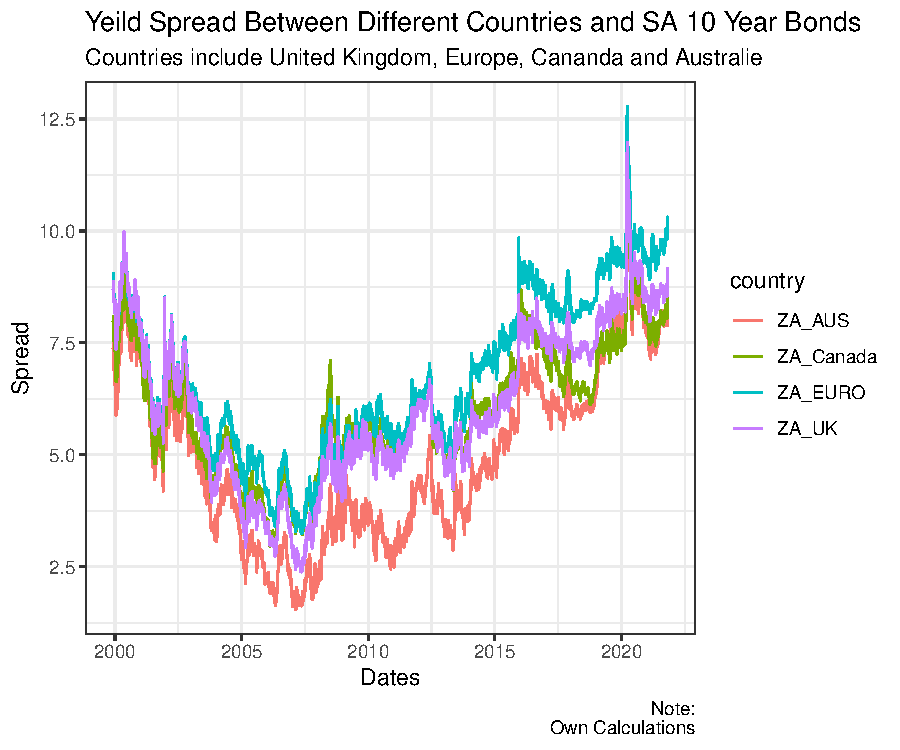
\includegraphics{Question1_files/figure-latex/unnamed-chunk-4-1.pdf}

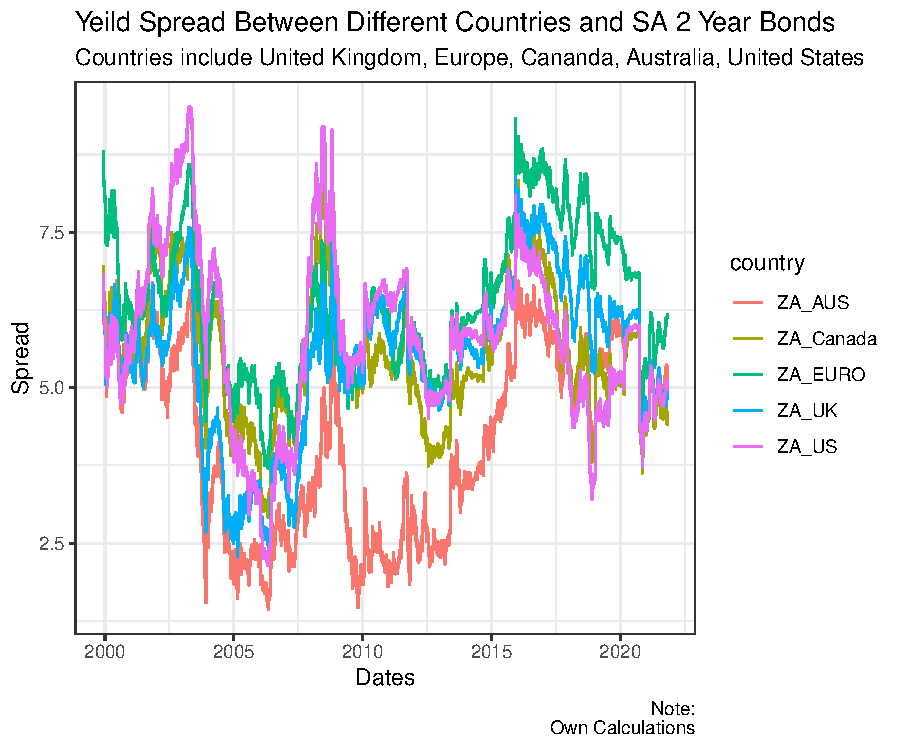
\includegraphics{Question1_files/figure-latex/unnamed-chunk-5-1.pdf}
\#\# Inflation In principle, the yield spread contains information on
expectations of future inflation that can be extracted as an estimate of
them. Studies of US and other markets have demonstrated that the yield
curve does contain information on expected and actual future levels of
gross domestic product (GDP) growth, and can be a lead indicator of
business cycle downturns.

Although many studies indicate the inflation-predicting power of the
yield curve in developed countries' markets, little is known of the
relationship in emerging economies. The graph below mostly supports the
notion that the yield spread contains valuable information about
expected inflation, where price refers to the inflation rate. However,
it is important to notice that inflation has much higher volatility then
yield spread. The graph below shows that the higher the current rate of
inflation, the higher the yields will rise across the yield curve, as
investors will demand this higher yield to compensate for inflation risk

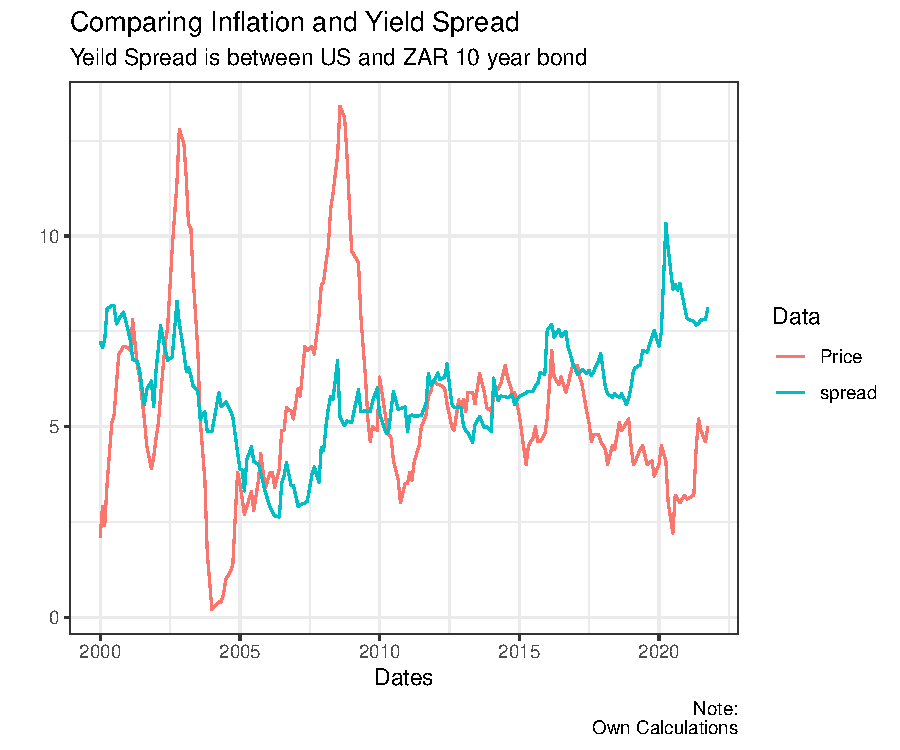
\includegraphics{Question1_files/figure-latex/unnamed-chunk-6-1.pdf}

\bibliography{Tex/ref}





\end{document}
